% IEEE Access manuscript package for DeepFirm Quant.
% Official template source: ACCESS_latex_template_20240429 from IEEE Access.
\documentclass{ieeeaccess}

\usepackage{cite}
\usepackage{amsmath,amssymb,amsfonts}
\usepackage{graphicx}
\usepackage{textcomp}
\usepackage{booktabs}
\usepackage{tabularx}
\usepackage{array}
\usepackage{url}

\graphicspath{{../../experiments/figures/}}
\newcolumntype{Y}{>{\raggedright\arraybackslash}X}
\newcommand{\tabnote}[1]{\vspace{2pt}\begin{flushleft}\footnotesize Note: #1\end{flushleft}}
\newcommand{\hashcell}[2]{\begin{tabular}[t]{@{}l@{}}#1\\#2\end{tabular}}
\makeatletter
\setlength{\@dblfptop}{0pt}
\makeatother
\def\BibTeX{{\rm B\kern-.05em{\sc i\kern-.025em b}\kern-.08em
    T\kern-.1667em\lower.7ex\hbox{E}\kern-.125emX}}

\begin{document}

\vol{14}
\year{2026}

\history{Submitted for review on May 18, 2026.}
\doi{To be assigned by IEEE Access}

\title{An Auditable Explainable AI Framework for Multi-Market Tail-Risk Warning and Leakage-Guarded Bayesian Portfolio Allocation}

\author{\uppercase{Hongyi Zhou}\authorrefmark{1}}
\address[1]{School of Professional Education and Executive Development, The Hong Kong Polytechnic University, Hong Kong (e-mail: p9112288@gmail.com)}
\tfootnote{This work received no external funding and was self-funded by the author.}
\markboth
{Zhou: Auditable Explainable AI for Multi-Market Tail-Risk Warning}
{Zhou: Auditable Explainable AI for Multi-Market Tail-Risk Warning}
\corresp{Corresponding author: Hongyi Zhou (e-mail: p9112288@gmail.com).}

\begin{abstract}
Financial machine-learning systems used in portfolio risk workflows often mix opaque predictions, fragile backtests, and unclear data provenance. That evidence is hard to audit when warning models, data providers, and allocation policies interact across markets.

This paper evaluates DeepFirm Quant as an auditable financial ML framework rather than a new predictive model. The system freezes crisis-warning artifacts, validates artifact and feature-schema hashes, records provenance and data-availability failures, prohibits sandbox substitution for paper metrics, reports native contribution drivers, and evaluates allocation policies under leakage-guarded as-of controls.

With sandbox data disabled, the frozen warning layer produced 68,324 predictions over 19 available holdout portfolios across US, Hong Kong, China A-share, Japan, and Taiwan markets. Aggregate ROC-AUC was 0.6325 for both 1D and 5D horizons, with PR-AUC of 0.1020 and 0.0904 and top-decile lifts of 2.30 and 1.90. In allocation OOS evaluation, Smart policy with the OOS guard had mean Sharpe ratio 1.1914 and model score 59.92, while mean benchmark excess return remained negative for every evaluated strategy.

Taken together, the results support audit review, probability-quality diagnostics, risk-ranking surveillance, and leakage-guarded decision discipline. They do not establish return prediction, positive benchmark excess return, causal market mechanisms, or investment advice.
\end{abstract}

\begin{keywords}
Financial machine learning, explainable AI, model risk management, tail-risk warning, portfolio allocation, Black-Litterman, out-of-sample validation.
\end{keywords}

\titlepgskip=-15pt
\maketitle

\section{Introduction}
\label{sec:introduction}
\PARstart{M}{achine-learning} methods are increasingly used in financial risk and portfolio workflows, but their deployment is constrained by four recurring problems. First, many models operate as black boxes whose risk warnings cannot be inspected by portfolio managers, model validators, or compliance reviewers. Second, apparently strong backtests are often contaminated by future-data leakage, including feature construction, benchmark alignment, model selection, or decision policies that observe data beyond their stated as-of date. Third, models trained on one market or asset sleeve may generalize weakly across regional trading calendars, liquidity regimes, and provider-specific data quality. Fourth, repeated strategy search can turn historical backtests into overfit demonstrations rather than credible out-of-sample (OOS) evidence \cite{White2000RealityCheck,BaileyEtAl2016BacktestOverfitting,BaileyLopezDePrado2014DeflatedSharpe,LopezDePrado2018FinancialML}.

This paper studies DeepFirm Quant as a research stack for auditable risk warning and allocation decision support. The crisis-warning module estimates whether a submitted portfolio is approaching a future tail-risk event at 1D or 5D horizons. It does not forecast exact returns. The allocation module evaluates Bayesian portfolio weights under Smart and Professional-style controls. The system is not an investment-advice system, and the reported OOS results should not be read as recommendations for any security, market, or strategy.

The paper asks a narrower question than whether one model can dominate a leaderboard: can a financial ML system still be useful when its forecasts are modest, if it behaves like an audit contract? Such a system must expose provenance, validate frozen artifacts, refuse silent sandbox substitution, separate probability quality from operating thresholds, guard allocation decisions against leakage, and report weak results plainly. For that reason, the paper focuses on auditability, explainability, and leakage-guarded evaluation rather than broad performance claims.

This audit-contract framing is motivated by supervisory model-risk guidance that separates disciplined model development, effective validation, and governance controls, but it should not be read as a claim that the research system satisfies regulatory compliance requirements \cite{FederalReserveOCC2011SR117ModelRisk}. The same control surface maps to the NIST AI RMF functions Govern, Map, Measure, and Manage through versioned artifact ownership, documented market/data scope, calibration and OOS measurements, and threshold or allocation guardrails \cite{Tabassi2023NISTAIRMF}. The reproducibility package is also aligned with IEEE Access artifact expectations by preserving code, data-access configuration, result files, environment notes, and execution instructions for independent review \cite{IEEEAccessReproducibility2026}.

The paper is organized around three research questions:
\begin{enumerate}
\item \textbf{RQ1: Audit contract.} Does an explicit audit contract improve reviewability by making artifacts, feature schemas, provenance failures, sandbox-use restrictions, and result hashes inspectable?
\item \textbf{RQ2: Frozen warning layer.} When frozen warning artifacts are applied to real multi-market holdout portfolios, what evidence do they provide for risk ranking, calibration, and threshold behavior?
\item \textbf{RQ3: Leakage-guarded allocation.} Does leakage-guarded allocation improve decision discipline under as-of constraints, without treating the policy as a guarantee of positive benchmark excess return?
\end{enumerate}

The contributions are:
\begin{enumerate}
\item An audit-contract formulation for financial ML that maps common failure modes to inspectable controls and reproducible evidence artifacts.
\item A frozen multi-market tail-risk warning setup with artifact hashes, feature-schema hashes, validation status, and model-version metadata.
\item A dynamic trailing-quantile tail-event construction designed to avoid direct look-ahead labeling.
\item SHAP-style feature contribution reporting for warning explanations, grounded in the XGBoost artifact's native contribution path \cite{ChenGuestrin2016XGBoost,LundbergLee2017SHAP}.
\item A leakage-guarded allocation evaluation that constrains Smart policy signals to the train window and verifies policy as-of dates.
\item A real-data applied validation over US, HK, CN, JP, and TW holdout portfolios, including threshold-sensitivity and ranking-surveillance diagnostics with explicit logs for unavailable provider data rather than synthetic substitution.
\end{enumerate}

\section{Related Work}
\label{sec:related}

\subsection{Financial Tail-Risk Forecasting}
Market-risk measurement has long used Value at Risk and related interval forecasts, with RiskMetrics providing an influential industry reference \cite{JPMorganReuters1996RiskMetricsTechnicalDocument}. Coherent risk-measure theory and Expected Shortfall/CVaR motivate downside-risk measures that address limitations of quantile-only risk summaries \cite{ArtznerEtAl1999CoherentRisk,RockafellarUryasev2000CVaR,AcerbiTasche2002ExpectedShortfall}. Econometric tail-risk forecasting includes interval forecast evaluation and conditional autoregressive VaR models \cite{Christoffersen1998IntervalForecasts,EngleManganelli2004CAViaR}. Recent financial ML work extends VaR and ES forecasting with forecast combinations, neural quantile regression, and neural-GARCH hybrids \cite{Taylor2020ForecastCombinationsVaRES,ChronopoulosEtAl2023DeepVaR,BuczynskiChlebus2023GARCHNet}.

\subsection{Explainable AI for Financial Risk}
Explainability is particularly important in financial risk management because decisions can affect capital allocation, risk limits, and client communication. SHAP provides additive feature-attribution explanations for model outputs \cite{LundbergLee2017SHAP}, while LIME and broader XAI taxonomies motivate local explanations and responsible AI framing \cite{RibeiroSinghGuestrin2016LIME,BarredoArrietaEtAl2020XAI}. Financial XAI work further argues for explanation mechanisms that can be inspected in fintech risk workflows \cite{BussmannEtAl2020XAIFintechRisk}.

\subsection{Black-Litterman and Bayesian Allocation}
Mean-variance optimization remains a foundation for portfolio construction \cite{Markowitz1952PortfolioSelection}. The Black-Litterman model combines equilibrium returns with investor views and view uncertainty, making it a natural Bayesian allocation layer for combining priors and model-driven signals \cite{BlackLitterman1992GlobalPortfolioOptimization,SatchellScowcroft2000BlackLittermanDemystification,Meucci2008BlackLittermanExtensions}. Recent work explores machine-learning and data-driven views within allocation pipelines \cite{BanElKarouiLim2018MLPortfolioOptimization,LiEtAl2022IntelligentBlackLitterman,BaruaSharma2022DynamicBlackLittermanMLViews,BaruaSharma2023FearGreedMLBlackLitterman}.

\subsection{OOS Validation and Leakage Awareness}
Financial ML is especially vulnerable to overfitting because researchers can search across assets, windows, labels, and strategy variants. Data-snooping tests, deflated performance measures, and purged or embargoed validation protocols are therefore central to credible evaluation \cite{White2000RealityCheck,BaileyEtAl2016BacktestOverfitting,BaileyLopezDePrado2014DeflatedSharpe,LopezDePrado2018FinancialML}. This paper follows the same spirit by freezing the crisis artifacts, logging data failures, and checking as-of dates for allocation decisions.

\subsection{Model Risk Governance and Reproducibility}
Model risk governance provides a complementary lens for evaluating financial AI systems. Federal Reserve SR 11-7 and OCC Bulletin 2011-12 organize model risk management around model development, implementation and use, validation, and governance policies and controls \cite{FederalReserveOCC2011SR117ModelRisk}. This paper uses that structure as motivation for its audit-contract controls, including frozen artifacts, schema validation, provenance logs, and leakage checks, without claiming supervisory compliance.

The NIST AI RMF 1.0 frames AI risk management through the Govern, Map, Measure, and Manage functions \cite{Tabassi2023NISTAIRMF}. At a research-system level, DeepFirm Quant connects those functions to concrete artifacts: governance through artifact contracts and logs, mapping through market scope and data-availability documentation, measurement through calibration, OOS, and uncertainty diagnostics, and management through conservative threshold interpretation and OOS allocation guards.

Reproducibility is also part of risk governance because independent reviewers need enough material to rerun or inspect the workflow. IEEE Access reproducibility instructions call for artifacts such as code, datasets or data-access descriptions, dependency requirements, installation/deployment instructions, benchmarks, test suites, and documentation \cite{IEEEAccessReproducibility2026}. The paper's reproducibility package records executable commands, frozen result files, hashes, skip logs, and environment notes.

\section{Framework}
\label{sec:framework}

\subsection{Data Ingestion and Provenance}
The framework supports standalone US, HK, CN, JP, and TW portfolio modes. The data layer records provider source details and data-quality warnings for each experiment. Yahoo Finance chart paths are used for several markets, while China A-share data can rely on AKShare and a Yahoo fallback where supported. The paper experiments require \texttt{allow\_sandbox\_data=false}; when a real provider fails, the portfolio or horizon is logged as unavailable rather than replaced with synthetic data.

\subsection{Market Calendar Alignment}
Portfolio prices are aligned by market-specific trading calendars and normalized into a common close-price contract. Benchmark returns are aligned to OOS test returns using date intersections first and only bounded forward fill where the experiment helper allows it. This avoids unbounded backfill and reduces the risk that benchmark comparisons use information unavailable on the test date.

\subsection{Feature Engineering}
For each portfolio, the risk engine builds point-in-time features including 1D and 5D portfolio returns, rolling volatility, rolling mean return, rolling drawdown, downside volatility, skewness, kurtosis, and correlation summaries. These features are computed from historical prices up to the current date. The frozen artifacts require a 14-feature schema; feature-schema hashes are recorded in Table~\ref{tab:artifact}.

\subsection{Tail-Event Label Construction}
The crisis-warning target is a dynamic trailing-quantile event. At horizon $h$, the label indicates whether the future $h$-day portfolio log return falls below a shifted trailing 5\% historical $h$-day return threshold:
\begin{equation}
y_{t,h}=\mathbf{1}\{r_{t+1:t+h}\leq q_{0.05,t,h}\}.
\end{equation}
This makes the prediction target a tail-event warning rather than a point return forecast.

\subsection{Frozen XGBoost Crisis-Warning Artifacts}
Two global artifacts are evaluated: \texttt{global\_h1} and \texttt{global\_h5}. The H1 artifact contains 36,849 training rows and 1,941 positive events; the H5 artifact contains 36,689 training rows and 2,102 positive events. Both cover US, HK, CN, JP, and TW and are marked globally complete, but both have \texttt{degraded\_validation} status in frozen metadata. The full SHA-256 hashes are preserved in the generated Markdown tables and result manifest; Table~\ref{tab:artifact} reports the audit-relevant values in submission format.

\begin{table*}[t]
\caption{Frozen Artifact Audit Summary}
\label{tab:artifact}
\centering
\scriptsize
\begin{tabularx}{\textwidth}{l l Y Y l l}
\toprule
Horizon & Model version & Artifact SHA-256 & Feature-schema SHA-256 & Validation & Match \\
\midrule
H1 & crisis-warning-xgb-h1-2026-05-17 & \hashcell{b807acefbc0c5774844331b7514791fd}{892f33a59846250728a64ca55506d6cd} & \hashcell{47b23430fb89b4626436b0e9dd3f14017}{183473c4af2450b25601fd935512ece} & degraded & true \\
H5 & crisis-warning-xgb-h5-2026-05-17 & \hashcell{625482ed714b903cd94ebdfd47fc8d9}{b0b0e7e5282ccc6a3b9af290b537053d0} & \hashcell{cc27ed4e44fbd4658e39591391e8a339}{a1d968fb35a94eb46417d2ee687260e9} & degraded & true \\
\bottomrule
\end{tabularx}
\tabnote{Frozen H1/H5 artifact directories were not retrained. Artifact and feature-schema hashes are validated against metadata before paper use; the table documents the audit contract rather than model performance.}
\end{table*}

\subsection{SHAP Explanations and Warning Levels}
The warning layer reports calibrated crisis probability, warning level, and top feature drivers. The SHAP-style driver table uses XGBoost native contribution values for recent holdout rows. These explanations should be interpreted as model-output attributions, not causal statements about market mechanisms.

\subsection{Smart Allocation Policy and Leakage Guard}
The allocation layer evaluates equal weight, inverse volatility, mean-variance, raw Black-Litterman, Smart policy, and Smart policy with OOS guard. Smart policy adjusts constraints and penalties from train-window risk state, regime, anomaly, and OOS diagnostics. The OOS guard checks underperformance and risk signals and may blend toward more balanced or defensive weights. In the generated allocation results, all Smart rows have \texttt{oos\_leakage\_guard=true}, and every \texttt{policy\_asof} precedes the first test date; no as-of violations were observed.

\subsection{Audit-Contract Controls}
The main contribution lies less in a particular estimator than in the controls around the estimators. Table~\ref{tab:audit-contract} maps the main reviewer-relevant failure modes to controls and evidence artifacts that can be inspected without trusting narrative claims.

Viewed through a model-risk lens, these controls correspond to development evidence (data contracts, feature schemas, frozen artifacts), validation evidence (calibration, OOS, uncertainty, and leakage tests), and governance evidence (provenance logs, sandbox refusal, and result manifests), in line with the structure of SR 11-7/OCC 2011-12 but not as a compliance attestation \cite{FederalReserveOCC2011SR117ModelRisk}. They also connect to AI RMF Govern, Map, Measure, and Manage functions through explicit ownership and policies, market/data context, quantitative diagnostics, and operational guardrails \cite{Tabassi2023NISTAIRMF}. The same evidence bundle helps artifact reviewers inspect the code, configuration, outputs, hashes, and execution instructions required for reproducibility \cite{IEEEAccessReproducibility2026}.

\begin{table*}[t]
\caption{Audit-Contract Controls}
\label{tab:audit-contract}
\centering
\scriptsize
\begin{tabularx}{\textwidth}{Y Y Y}
\toprule
Failure mode & Framework control & Evidence artifact, test, or log \\
\midrule
Artifact drift or silent retraining & Frozen \texttt{global\_h1} and \texttt{global\_h5} directories; artifact hash validation against metadata & Table~\ref{tab:artifact}, \texttt{artifact\_audit\_summary.json}, \texttt{validate\_crisis\_warning\_contract.py} \\
Feature-schema drift & Feature-schema hash validation and fixed 14-feature contract & Feature-schema hash fields in artifact metadata and Table~\ref{tab:artifact} \\
Synthetic data substitution & Paper commands require sandbox data disabled; provider failures are logged as skips & \texttt{paper\_eval\_config.yaml}, data-availability log, skipped CSV files \\
Opaque warning output & Native XGBoost contribution rows for recent holdout observations & \texttt{crisis\_shap\_drivers.csv}, Fig.~\ref{fig:shap} \\
Future-data leakage in allocation & Train-window policy state, OOS guard flag, and \texttt{policy\_asof} checks & \texttt{test\_oos\_allocation\_integrity.py}, \texttt{allocation\_oos\_metrics.csv} \\
Threshold overclaiming & Threshold grid and top-percentile ranking surveillance metrics & Table~\ref{tab:threshold}, Fig.~\ref{fig:threshold} \\
Provider coverage gaps & Data availability log and skipped-row CSVs; no silent replacement & \texttt{crisis\_eval\_skipped.csv}, \texttt{allocation\_oos\_skipped.csv} \\
\bottomrule
\end{tabularx}
\end{table*}

\begin{figure*}[t]
  \centering
  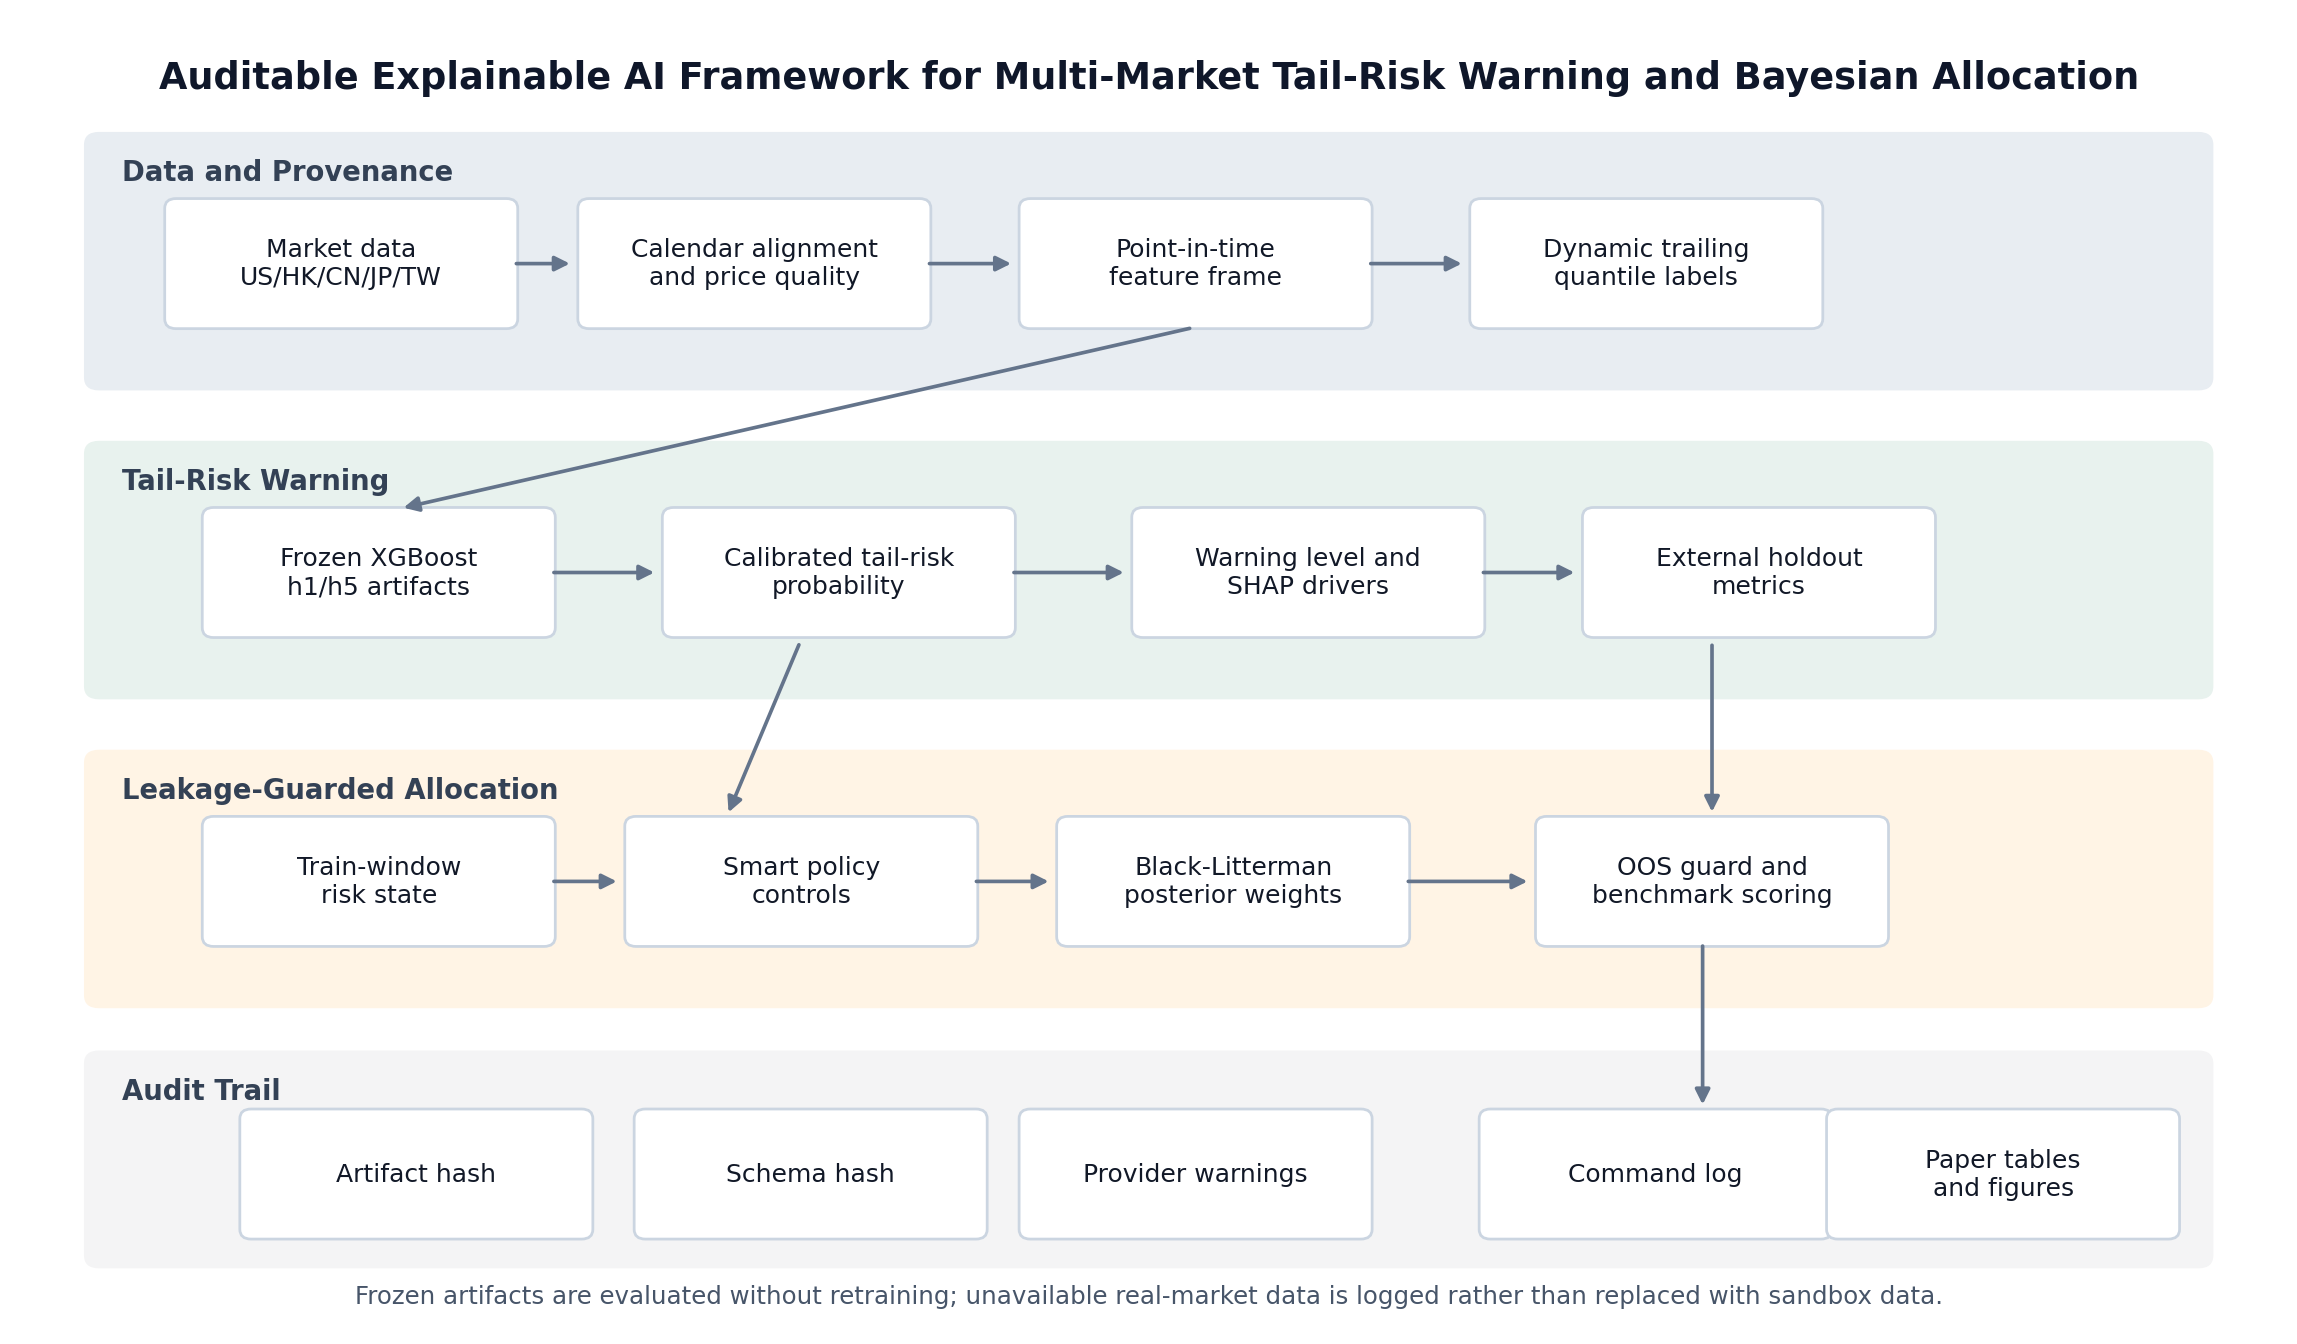
\includegraphics[width=0.95\textwidth]{framework_architecture.png}
  \caption{Auditable DeepFirm Quant workflow from real-market data ingestion through frozen H1/H5 crisis-warning artifacts, SHAP-style explanation, leakage-guarded allocation, and paper outputs. Sandbox substitution is disabled for paper metrics, and skipped provider data is logged rather than imputed.}
  \label{fig:framework}
\end{figure*}

\section{Experimental Protocol}
\label{sec:protocol}

\subsection{Frozen Artifact Setup}
The paper uses the existing \path{artifacts/crisis_warning/global_h1/} and \path{artifacts/crisis_warning/global_h5/} directories. The crisis-warning artifact contract validation command passed before experiments. The experiment framework tests passed, and the crisis-warning/OOS/provenance integrity suite had previously passed as part of the manuscript worklog.

\subsection{Holdout Portfolio Construction}
The holdout pool contains 20 portfolios, 4 per market. Exact same-market duplicate ticker-set count versus the training-domain portfolios is zero. Several portfolios share individual constituents with the training domain, with maximum within-market overlap of 3 out of 5 tickers. The evaluation is therefore portfolio-level external validation, not a zero-security-overlap transfer test.

A separate zero-security-overlap crisis-warning supplement is provided in the supplement portfolio file. It contains 10 portfolios, two per market, selected after checking frozen training-domain tickers from artifact metadata. This supplement is reported separately so the main evaluation remains comparable to the original 20-portfolio holdout design.

\subsection{Baselines}
Crisis-warning baselines are evaluated on the final 20\% of each available holdout portfolio. Logistic regression, random forest, and gradient boosting baselines are trained only on the first 80\% of that portfolio's point-in-time feature rows. A historical-tail-threshold baseline predicts warning when the current historical horizon return breaches the current tail threshold. The frozen calibrated and raw XGBoost outputs are sliced to the same test windows for comparison.

Allocation baselines include equal weight, inverse volatility, mean-variance, raw Black-Litterman, Smart policy, and Smart policy with OOS guard.

\subsection{Metrics}
Crisis-warning metrics include row count, positive event count, positive rate, ROC-AUC, PR-AUC, Brier score, log-loss, calibration error, precision and recall at 0.60, and top-decile lift. Because tail events are rare, PR-AUC and top-percentile ranking metrics are more operationally informative than ROC-AUC alone. Threshold sensitivity is computed at 0.05, 0.075, 0.10, 0.15, 0.20, 0.30, 0.40, 0.50, and 0.60, with precision, recall, F1, flag rate, flag count, and positive count reported globally, by horizon, by market, and by horizon-market group. Ranking surveillance metrics report top 1\%, top 5\%, and top 10\% precision, recall, and lift. Allocation metrics include cumulative return, benchmark cumulative return, benchmark excess return, annualized volatility, max drawdown, Expected Shortfall, Sharpe ratio, Information Ratio, turnover, model score, and model grade.

\subsection{Failure Handling}
Real-data provider failures are logged in the data-availability log. The main crisis external evaluation skipped \texttt{cn\_broad\_factor\_etf} for both horizons because ticker \texttt{159915} could not be fetched. The refreshed baseline comparison uses the same available real-data cache and also skips only \texttt{cn\_broad\_factor\_etf}. Allocation OOS skipped \texttt{cn\_broad\_factor\_etf}. These omissions are data availability limitations.

\section{Results}
\label{sec:results}

\subsection{Artifact Audit Summary}
Table~\ref{tab:artifact} and Fig.~\ref{fig:framework} summarize the audit surface. Both frozen artifacts passed hash validation. The artifact audit summary confirms that the computed H1 and H5 artifact hashes match metadata. Both artifacts are globally complete across the five target markets, but the frozen validation status is \texttt{degraded\_validation}. That status is acceptable for studying auditability; it is not evidence of strong predictive reliability.

\subsection{Crisis Warning External Evaluation}
With sandbox data disabled and network-enabled real-market fetching, the crisis external evaluation produced 68,324 prediction rows and 2 skipped rows. Table~\ref{tab:crisis} reports the market-level breakdown, and Fig.~\ref{fig:roc-pr} plots ROC and PR behavior by horizon.

\begin{table*}[t]
\caption{Crisis Warning External Metrics by Market}
\label{tab:crisis}
\centering
\scriptsize
\begin{tabularx}{\textwidth}{c c r r r r r r r r r}
\toprule
H & Market & Rows & Pos. & ROC & PR & Brier & Log-loss & Prec@0.60 & Recall@0.60 & Top-decile lift \\
\midrule
1 & CN & 5,700 & 272 & 0.5863 & 0.0786 & 0.0451 & 0.1952 & 0.5000 & 0.0074 & 1.9485 \\
1 & HK & 5,782 & 315 & 0.5984 & 0.0946 & 0.0508 & 0.2095 & 0.0000 & 0.0000 & 2.2192 \\
1 & JP & 7,886 & 431 & 0.6391 & 0.1025 & 0.0506 & 0.2041 & 0.0000 & 0.0000 & 2.5045 \\
1 & TW & 6,702 & 385 & 0.6348 & 0.1057 & 0.0530 & 0.2123 & 1.0000 & 0.0026 & 2.5165 \\
1 & US & 8,168 & 437 & 0.6730 & 0.1249 & 0.0491 & 0.2024 & 0.6000 & 0.0069 & 2.4937 \\
5 & CN & 5,676 & 277 & 0.6268 & 0.0815 & 0.0458 & 0.1900 & 0.0000 & 0.0000 & 2.2006 \\
5 & HK & 5,750 & 330 & 0.5699 & 0.0959 & 0.0533 & 0.2240 & 0.0000 & 0.0000 & 2.1212 \\
5 & JP & 7,854 & 467 & 0.6339 & 0.0932 & 0.0552 & 0.2339 & 0.0000 & 0.0000 & 2.2895 \\
5 & TW & 6,670 & 404 & 0.6526 & 0.0944 & 0.0564 & 0.2233 & 0.0000 & 0.0000 & 2.1287 \\
5 & US & 8,136 & 452 & 0.6611 & 0.0949 & 0.0517 & 0.2139 & 0.0000 & 0.0000 & 2.0786 \\
\bottomrule
\end{tabularx}
\tabnote{Metrics use 68,324 real-data holdout predictions with sandbox disabled across 1D and 5D horizons. Two skipped crisis-warning rows were logged for \texttt{cn\_broad\_factor\_etf}. PR-AUC is emphasized alongside ROC-AUC because tail events are rare.}
\end{table*}

Aggregated over available holdout portfolios, H1 has 34,238 rows, 1,840 positives, ROC-AUC 0.6325, PR-AUC 0.1020, Brier 0.0498, log-loss 0.2047, calibration error 0.0018, precision@0.60 0.5455, recall@0.60 0.0033, and top-decile lift 2.2988. H5 has 34,086 rows, 1,930 positives, ROC-AUC 0.6325, PR-AUC 0.0904, Brier 0.0527, log-loss 0.2181, calibration error 0.0035, precision@0.60 0.0000, recall@0.60 0.0000, and top-decile lift 1.9013.

\begin{figure*}[t]
  \centering
  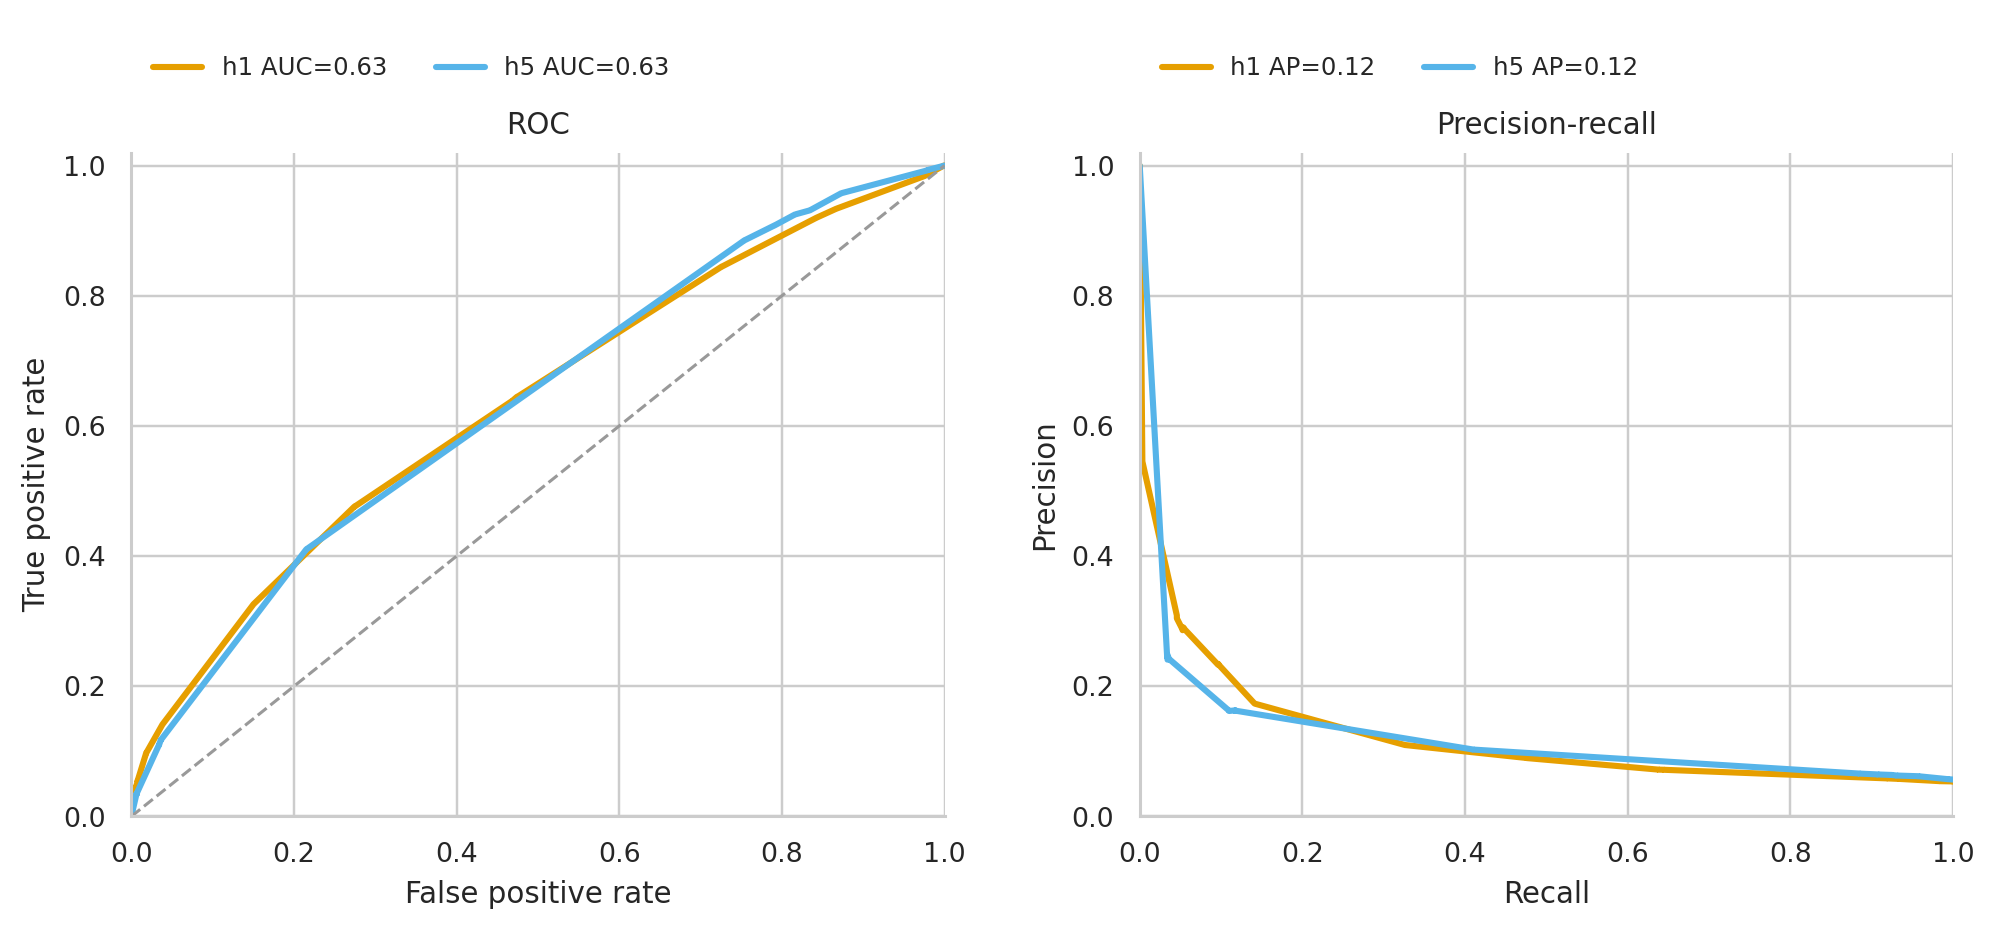
\includegraphics[width=0.95\textwidth]{roc_pr_by_horizon.png}
  \caption{ROC and precision-recall curves for 68,324 real-data holdout crisis predictions with sandbox disabled across 1D and 5D horizons. The precision-recall panel is more informative for rare tail events than ROC alone.}
  \label{fig:roc-pr}
\end{figure*}

\begin{figure*}[t]
  \centering
  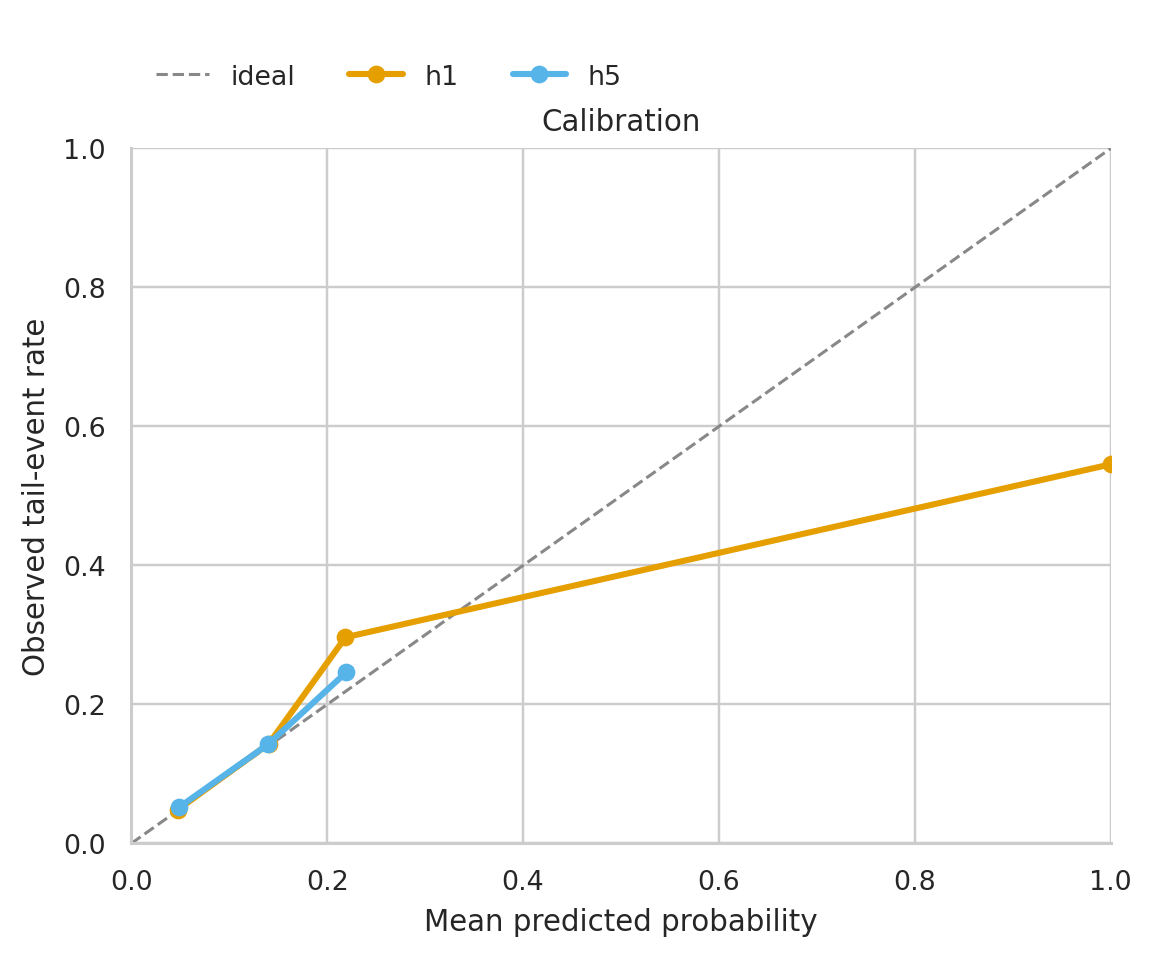
\includegraphics[width=0.78\textwidth]{calibration_by_horizon.png}
  \caption{Calibration curves for the same real-data H1/H5 holdout predictions. The figure evaluates probability quality, not the operational threshold; threshold selection is analyzed separately in Table~\ref{tab:threshold} and Fig.~\ref{fig:threshold}.}
  \label{fig:calibration}
\end{figure*}

\subsection{Threshold Sensitivity and Ranking Surveillance}
Table~\ref{tab:threshold} and Fig.~\ref{fig:threshold} make the threshold problem explicit. Globally, threshold 0.05 flags 61.88\% of rows and recalls 76.45\% of positives, but precision is only 6.82\%. Threshold 0.10 reduces the flag rate to 4.23\% with precision 16.81\%, recall 12.89\%, and F1 14.59\%. Threshold 0.20 flags only 0.79\% of rows with precision 27.68\% and recall 3.98\%. At 0.60, the model flags only 11 of 68,324 rows; global recall falls to 0.16\%, and H5 produces no flags. That threshold is therefore too sparse for a recall-sensitive crisis trigger.

A more defensible operational reading is ranking surveillance. Across both horizons, the top 1\% bucket has 26.02\% precision and 4.72 lift, the top 5\% bucket has 15.54\% precision and 2.82 lift, and the top 10\% bucket has 12.09\% precision, 21.91\% recall, and 2.19 lift. These values fit a watchlist or surveillance queue that sends high-score portfolios to review. They do not support a standalone binary alarm at 0.60.

\begin{table*}[t]
\caption{Threshold Sensitivity and Ranking Surveillance}
\label{tab:threshold}
\centering
\scriptsize
\begin{tabularx}{\textwidth}{l c c r r r r r r r r r}
\toprule
Scope & H & Threshold & Rows & Flag rate & Flags & Precision & Recall & F1 & Top10 precision & Top10 recall & Top10 lift \\
\midrule
Global & -- & 0.050 & 68,324 & 0.6188 & 42,277 & 0.0682 & 0.7645 & 0.1252 & 0.1209 & 0.2191 & 2.1908 \\
Global & -- & 0.075 & 68,324 & 0.1005 & 6,864 & 0.1205 & 0.2194 & 0.1555 & 0.1209 & 0.2191 & 2.1908 \\
Global & -- & 0.100 & 68,324 & 0.0423 & 2,891 & 0.1681 & 0.1289 & 0.1459 & 0.1209 & 0.2191 & 2.1908 \\
Global & -- & 0.150 & 68,324 & 0.0152 & 1,038 & 0.2360 & 0.0650 & 0.1019 & 0.1209 & 0.2191 & 2.1908 \\
Global & -- & 0.200 & 68,324 & 0.0079 & 542 & 0.2768 & 0.0398 & 0.0696 & 0.1209 & 0.2191 & 2.1908 \\
Global & -- & 0.300 & 68,324 & 0.0002 & 11 & 0.5455 & 0.0016 & 0.0032 & 0.1209 & 0.2191 & 2.1908 \\
Global & -- & 0.400 & 68,324 & 0.0002 & 11 & 0.5455 & 0.0016 & 0.0032 & 0.1209 & 0.2191 & 2.1908 \\
Global & -- & 0.500 & 68,324 & 0.0002 & 11 & 0.5455 & 0.0016 & 0.0032 & 0.1209 & 0.2191 & 2.1908 \\
Global & -- & 0.600 & 68,324 & 0.0002 & 11 & 0.5455 & 0.0016 & 0.0032 & 0.1209 & 0.2191 & 2.1908 \\
Horizon & 1 & 0.050 & 34,238 & 0.4770 & 16,332 & 0.0719 & 0.6380 & 0.1292 & 0.1203 & 0.2239 & 2.2390 \\
Horizon & 1 & 0.075 & 34,238 & 0.1597 & 5,468 & 0.1097 & 0.3261 & 0.1642 & 0.1203 & 0.2239 & 2.2390 \\
Horizon & 1 & 0.100 & 34,238 & 0.0438 & 1,500 & 0.1733 & 0.1413 & 0.1557 & 0.1203 & 0.2239 & 2.2390 \\
Horizon & 1 & 0.150 & 34,238 & 0.0222 & 761 & 0.2339 & 0.0967 & 0.1369 & 0.1203 & 0.2239 & 2.2390 \\
Horizon & 1 & 0.200 & 34,238 & 0.0080 & 274 & 0.3066 & 0.0457 & 0.0795 & 0.1203 & 0.2239 & 2.2390 \\
Horizon & 1 & 0.300 & 34,238 & 0.0003 & 11 & 0.5455 & 0.0033 & 0.0065 & 0.1203 & 0.2239 & 2.2390 \\
Horizon & 1 & 0.400 & 34,238 & 0.0003 & 11 & 0.5455 & 0.0033 & 0.0065 & 0.1203 & 0.2239 & 2.2390 \\
Horizon & 1 & 0.500 & 34,238 & 0.0003 & 11 & 0.5455 & 0.0033 & 0.0065 & 0.1203 & 0.2239 & 2.2390 \\
Horizon & 1 & 0.600 & 34,238 & 0.0003 & 11 & 0.5455 & 0.0033 & 0.0065 & 0.1203 & 0.2239 & 2.2390 \\
Horizon & 5 & 0.050 & 34,086 & 0.7612 & 25,945 & 0.0658 & 0.8850 & 0.1225 & 0.1185 & 0.2093 & 2.0930 \\
Horizon & 5 & 0.075 & 34,086 & 0.0410 & 1,396 & 0.1626 & 0.1176 & 0.1365 & 0.1185 & 0.2093 & 2.0930 \\
Horizon & 5 & 0.100 & 34,086 & 0.0408 & 1,391 & 0.1625 & 0.1171 & 0.1361 & 0.1185 & 0.2093 & 2.0930 \\
Horizon & 5 & 0.150 & 34,086 & 0.0081 & 277 & 0.2419 & 0.0347 & 0.0607 & 0.1185 & 0.2093 & 2.0930 \\
Horizon & 5 & 0.200 & 34,086 & 0.0079 & 268 & 0.2463 & 0.0342 & 0.0601 & 0.1185 & 0.2093 & 2.0930 \\
Horizon & 5 & 0.300 & 34,086 & 0.0000 & 0 & 0.0000 & 0.0000 & 0.0000 & 0.1185 & 0.2093 & 2.0930 \\
Horizon & 5 & 0.400 & 34,086 & 0.0000 & 0 & 0.0000 & 0.0000 & 0.0000 & 0.1185 & 0.2093 & 2.0930 \\
Horizon & 5 & 0.500 & 34,086 & 0.0000 & 0 & 0.0000 & 0.0000 & 0.0000 & 0.1185 & 0.2093 & 2.0930 \\
Horizon & 5 & 0.600 & 34,086 & 0.0000 & 0 & 0.0000 & 0.0000 & 0.0000 & 0.1185 & 0.2093 & 2.0930 \\
\bottomrule
\end{tabularx}
\tabnote{Computed from 68,324 real-data holdout crisis prediction rows with sandbox disabled. The 0.60 threshold is a conservative operating point; top-percentile columns summarize ranking surveillance behavior.}
\end{table*}

\begin{figure*}[t]
  \centering
  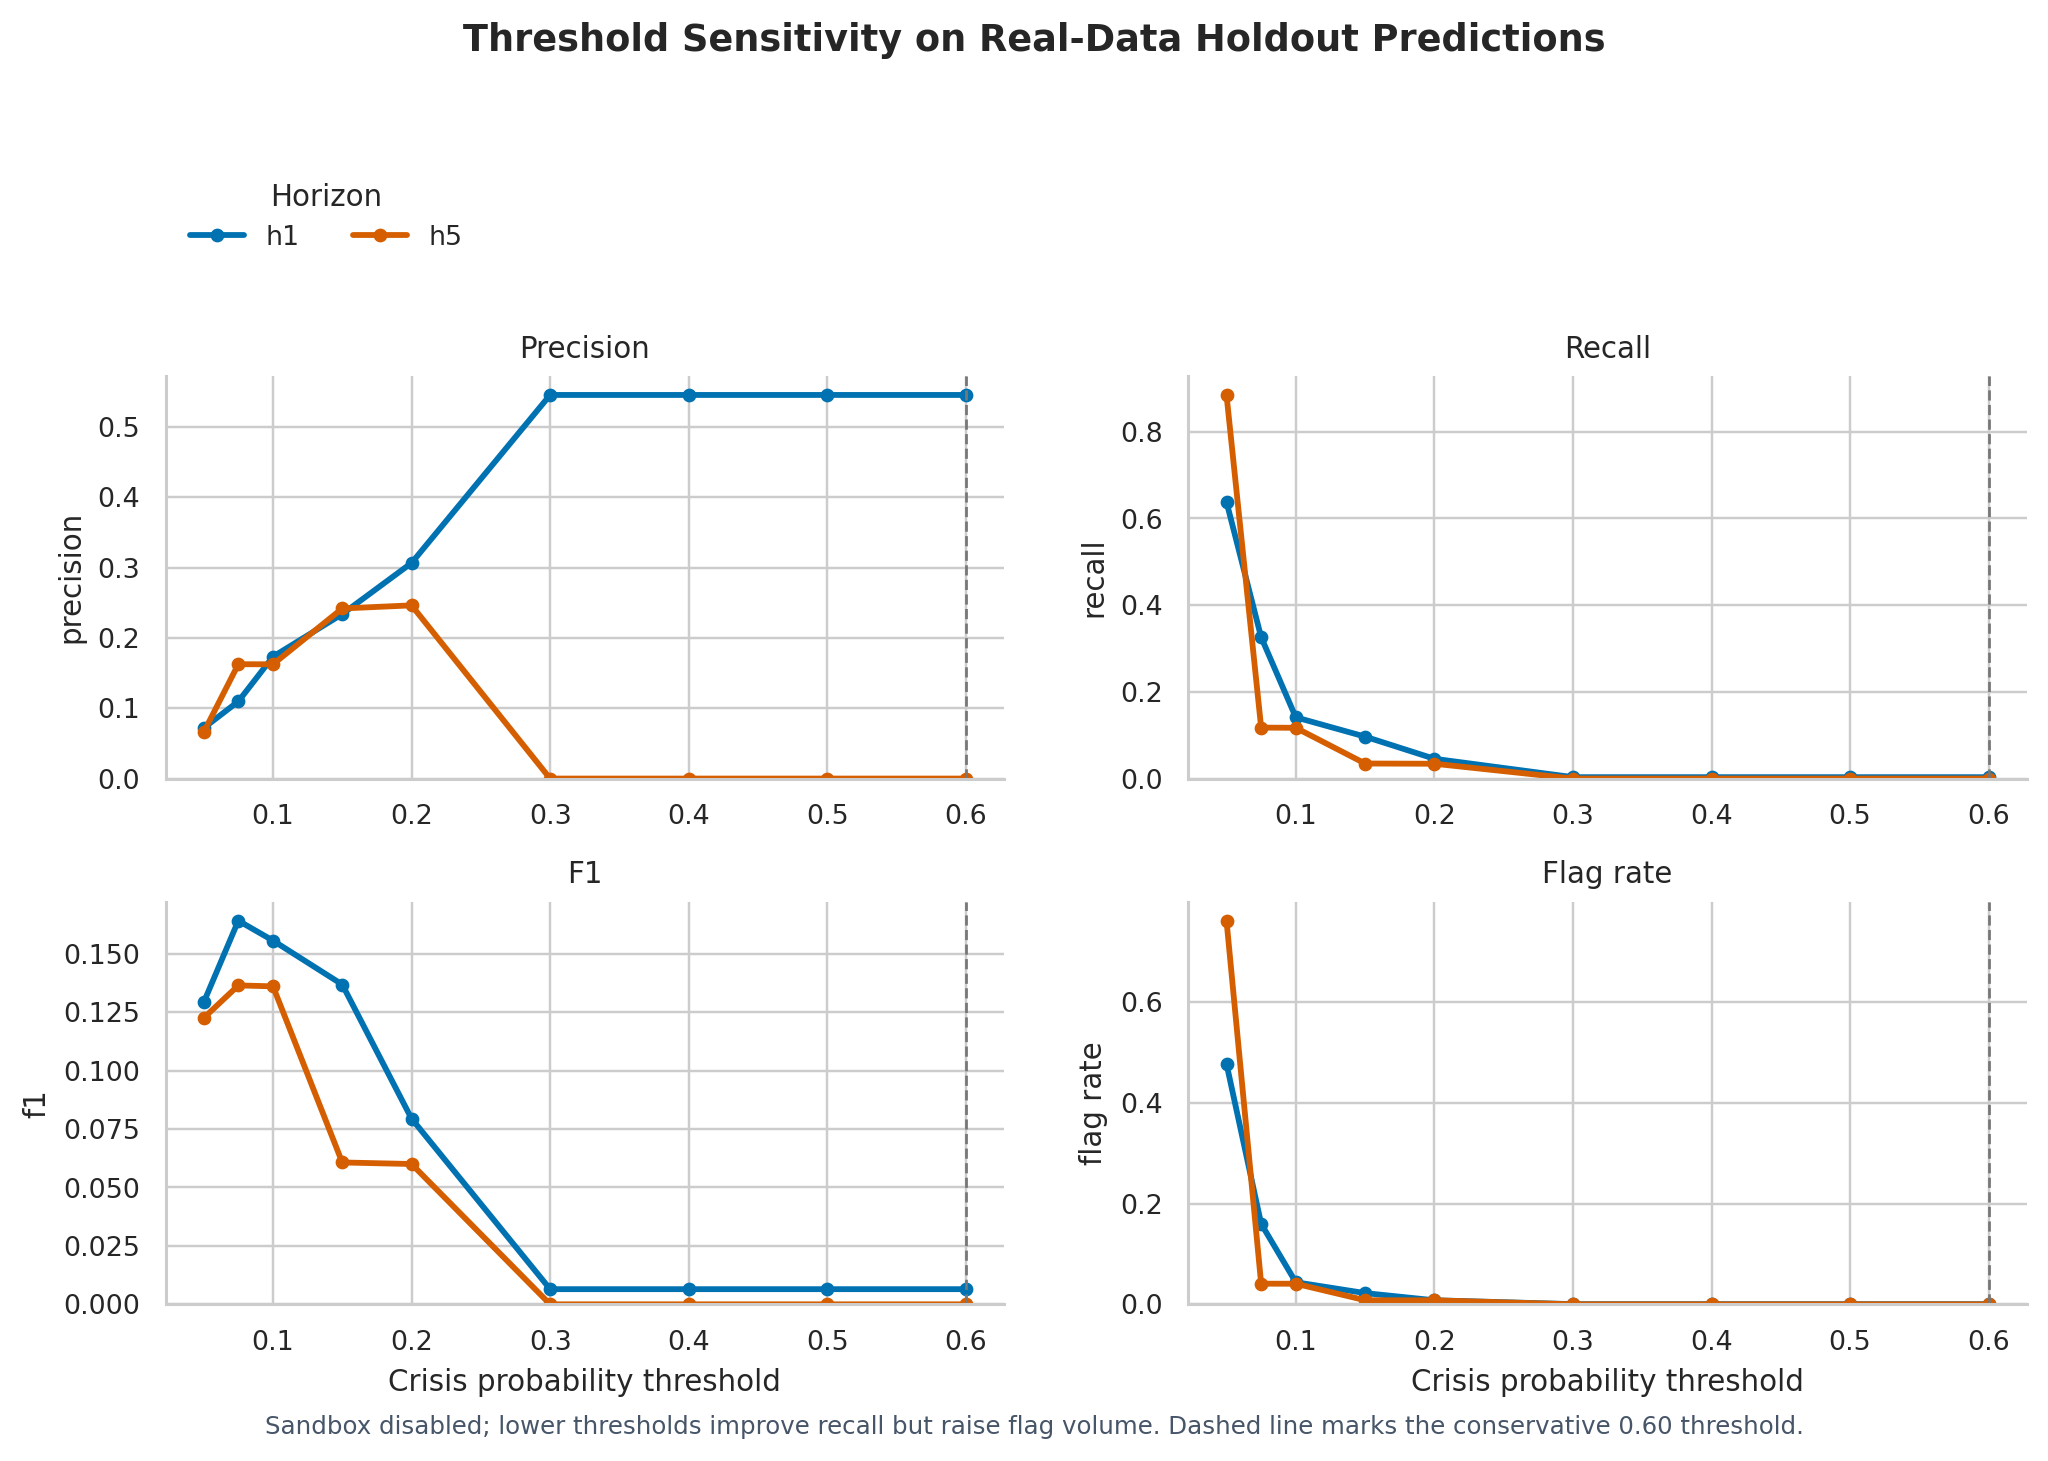
\includegraphics[width=0.88\textwidth]{threshold_sensitivity.png}
  \caption{Threshold sensitivity for real-data holdout predictions with sandbox disabled. The 0.60 operating point is conservative; lower thresholds recover recall only by increasing flag volume, so the evidence better supports ranking surveillance than a fixed binary trigger.}
  \label{fig:threshold}
\end{figure*}

\subsection{Zero-Security-Overlap Transfer Check}
A zero-security-overlap transfer-check portfolio file was constructed by checking every recommended ticker against the frozen training-domain tickers in \texttt{global\_h1} metadata. It contains 10 portfolios, two per market, with zero same-market security overlap. Running the frozen crisis artifacts on this transfer check with sandbox disabled produced 36,114 prediction rows and zero skipped rows. Baseline comparison, allocation OOS, and allocation ablation were not run for this panel; therefore, the zero-security-overlap evidence is limited to crisis-warning transfer behavior. The transfer-check results are consistent with the main evaluation: H1 achieved ROC-AUC 0.6290, PR-AUC 0.0971, Brier 0.0480, recall@0.60 0.0043, and top-decile lift 2.3551; H5 achieved ROC-AUC 0.6139, PR-AUC 0.0895, Brier 0.0534, recall@0.60 0.0000, and top-decile lift 1.8100. This transfer check reduces the ticker-overlap attack surface, but it does not change the main interpretation.

\subsection{Baseline Comparison}
Table~\ref{tab:baseline} reports the final-20\% baseline comparison, which produced 82,086 prediction rows and 300 metric rows with sandbox disabled. For H1, frozen calibrated XGBoost achieved ROC-AUC 0.6055 and PR-AUC 0.0905, while raw XGBoost achieved slightly higher ROC-AUC 0.6095 and PR-AUC 0.0992. The calibration layer substantially improved Brier score and log-loss: calibrated XGBoost had Brier/log-loss of 0.0504/0.2055, compared with 0.2084/0.6081 for raw XGBoost.

The same pattern appears at H5. Raw XGBoost had higher ROC-AUC (0.6122 versus 0.6014), but calibrated XGBoost had much lower Brier/log-loss (0.0460/0.1914 versus 0.2066/0.6012). The baseline comparison is therefore not a single leaderboard. Calibration improves probability quality, raw margins preserve stronger ranking in parts of this sample, and non-XGBoost baselines vary by horizon and metric.

\begin{table*}[t]
\caption{Crisis Baseline Comparison}
\label{tab:baseline}
\centering
\scriptsize
\begin{tabularx}{\textwidth}{c Y r r r r r r r r}
\toprule
H & Baseline & Rows & Pos. & ROC & PR & Brier & Log-loss & Recall@0.60 & Lift \\
\midrule
1 & frozen calibrated XGBoost & 6,858 & 371 & 0.6055 & 0.0905 & 0.0504 & 0.2055 & 0.0027 & 2.0210 \\
1 & frozen raw XGBoost & 6,858 & 371 & 0.6095 & 0.0992 & 0.2084 & 0.6081 & 0.2022 & 2.0479 \\
1 & gradient boosting & 6,858 & 371 & 0.5414 & 0.0594 & 0.0875 & 0.3211 & 0.0458 & 0.9970 \\
1 & historical tail threshold & 6,858 & 371 & 0.5245 & 0.0588 & 0.0967 & 2.0034 & 0.0997 & 1.4551 \\
1 & logistic regression & 6,858 & 371 & 0.5558 & 0.0713 & 0.2405 & 0.6818 & 0.2399 & 1.4551 \\
1 & random forest & 6,858 & 371 & 0.5759 & 0.0880 & 0.1140 & 0.3950 & 0.0431 & 1.7785 \\
5 & frozen calibrated XGBoost & 6,823 & 331 & 0.6014 & 0.0642 & 0.0460 & 0.1914 & 0.0000 & 2.0523 \\
5 & frozen raw XGBoost & 6,823 & 331 & 0.6122 & 0.0726 & 0.2066 & 0.6012 & 0.2024 & 1.8712 \\
5 & gradient boosting & 6,823 & 331 & 0.5717 & 0.0605 & 0.0668 & 0.2681 & 0.0423 & 1.2978 \\
5 & historical tail threshold & 6,823 & 331 & 0.5055 & 0.0491 & 0.0898 & 1.8618 & 0.0574 & 1.0563 \\
5 & logistic regression & 6,823 & 331 & 0.5501 & 0.0557 & 0.2404 & 0.6844 & 0.2598 & 1.0865 \\
5 & random forest & 6,823 & 331 & 0.5706 & 0.0752 & 0.0998 & 0.3568 & 0.0332 & 1.7807 \\
\bottomrule
\end{tabularx}
\tabnote{Baseline rows use real-data final-window holdout predictions with sandbox disabled. Non-frozen baselines train on the first 80\% of each available portfolio and evaluate on the final 20\%; frozen XGBoost is sliced to the same windows for fairness.}
\end{table*}

\subsection{Calibration and Interpretability}
Figure~\ref{fig:calibration} and the Brier/log-loss results support the use of a probability calibration layer when the output is used as a warning probability. Calibration is not the same as selecting an operating threshold: a probability model can be reasonably calibrated while a fixed trigger still has poor recall. Figure~\ref{fig:shap} ranks the most influential features by mean absolute native contribution in the SHAP-style driver output. These drivers are useful for audit review and user communication, but they should not be interpreted as causal stress tests.

\begin{figure*}[t]
  \centering
  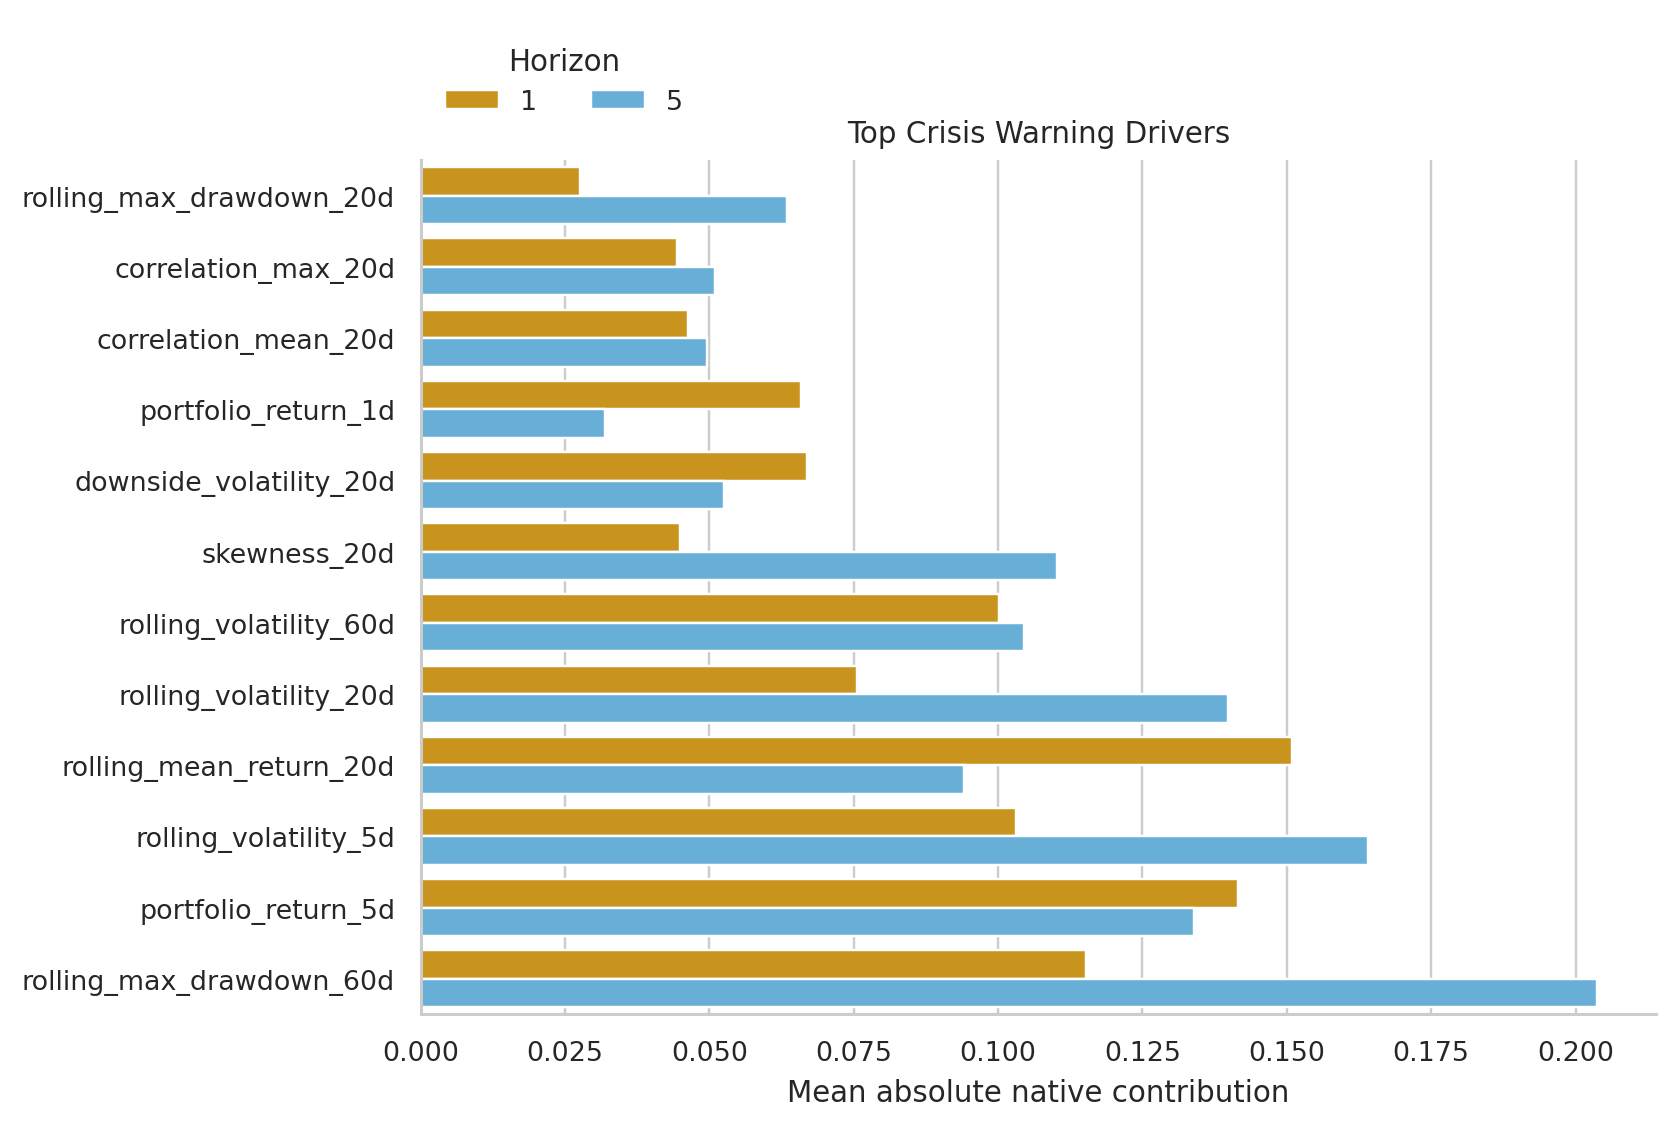
\includegraphics[width=0.88\textwidth]{shap_top_drivers.png}
  \caption{Mean absolute native XGBoost contribution values for recent holdout warning rows across H1 and H5 artifacts. The drivers support audit review and user communication, but they are not causal market stress-test variables.}
  \label{fig:shap}
\end{figure*}

\subsection{Allocation OOS Performance}
Table~\ref{tab:allocation} and Fig.~\ref{fig:allocation} summarize the allocation OOS evaluation, which covered 19 portfolios, 114 strategy rows, and 42,420 return rows with sandbox disabled. Smart policy with OOS guard had mean Sharpe 1.1914 and model score 59.92 in this run, and its mean turnover (0.3701) was far below Smart policy without the guard (1.6630) and raw Black-Litterman (1.7086). Nevertheless, all strategies had negative mean benchmark excess return, with Smart policy plus guard least negative at -0.1363. The allocation result therefore speaks to guarded decision discipline, not positive benchmark excess return.

\begin{table*}[t]
\caption{Allocation OOS Performance}
\label{tab:allocation}
\centering
\scriptsize
\begin{tabularx}{\textwidth}{Y r r r r r r r r r}
\toprule
Strategy & Port. & Cum. ret. & Vol. & Max DD & ES & Sharpe & IR & Turnover & Bench. excess \\
\midrule
Equal weight & 19 & 0.3763 & 0.2226 & -0.1974 & -0.0524 & 1.1203 & -0.4597 & 0.0000 & -0.1526 \\
Inverse volatility & 19 & 0.3355 & 0.2235 & -0.1955 & -0.0538 & 1.1255 & -0.4645 & 0.3152 & -0.1934 \\
Mean-variance & 19 & 0.4061 & 0.2389 & -0.2082 & -0.0560 & 1.1799 & -0.1963 & 2.4759 & -0.1228 \\
Raw Black-Litterman & 19 & 0.3738 & 0.2200 & -0.1937 & -0.0520 & 1.1581 & -0.3219 & 1.7086 & -0.1551 \\
Smart policy & 19 & 0.3732 & 0.2201 & -0.1939 & -0.0520 & 1.1531 & -0.3488 & 1.6630 & -0.1557 \\
Smart policy + OOS guard & 19 & 0.3926 & 0.2192 & -0.1919 & -0.0517 & 1.1914 & -0.3138 & 0.3701 & -0.1363 \\
\bottomrule
\end{tabularx}
\tabnote{Values are means across 19 real-data holdout portfolios, 114 strategy rows, and 42,420 OOS return rows with sandbox disabled. One allocation row was skipped for \texttt{cn\_broad\_factor\_etf}. Benchmark excess return remains negative for every listed strategy.}
\end{table*}

\begin{figure*}[t]
  \centering
  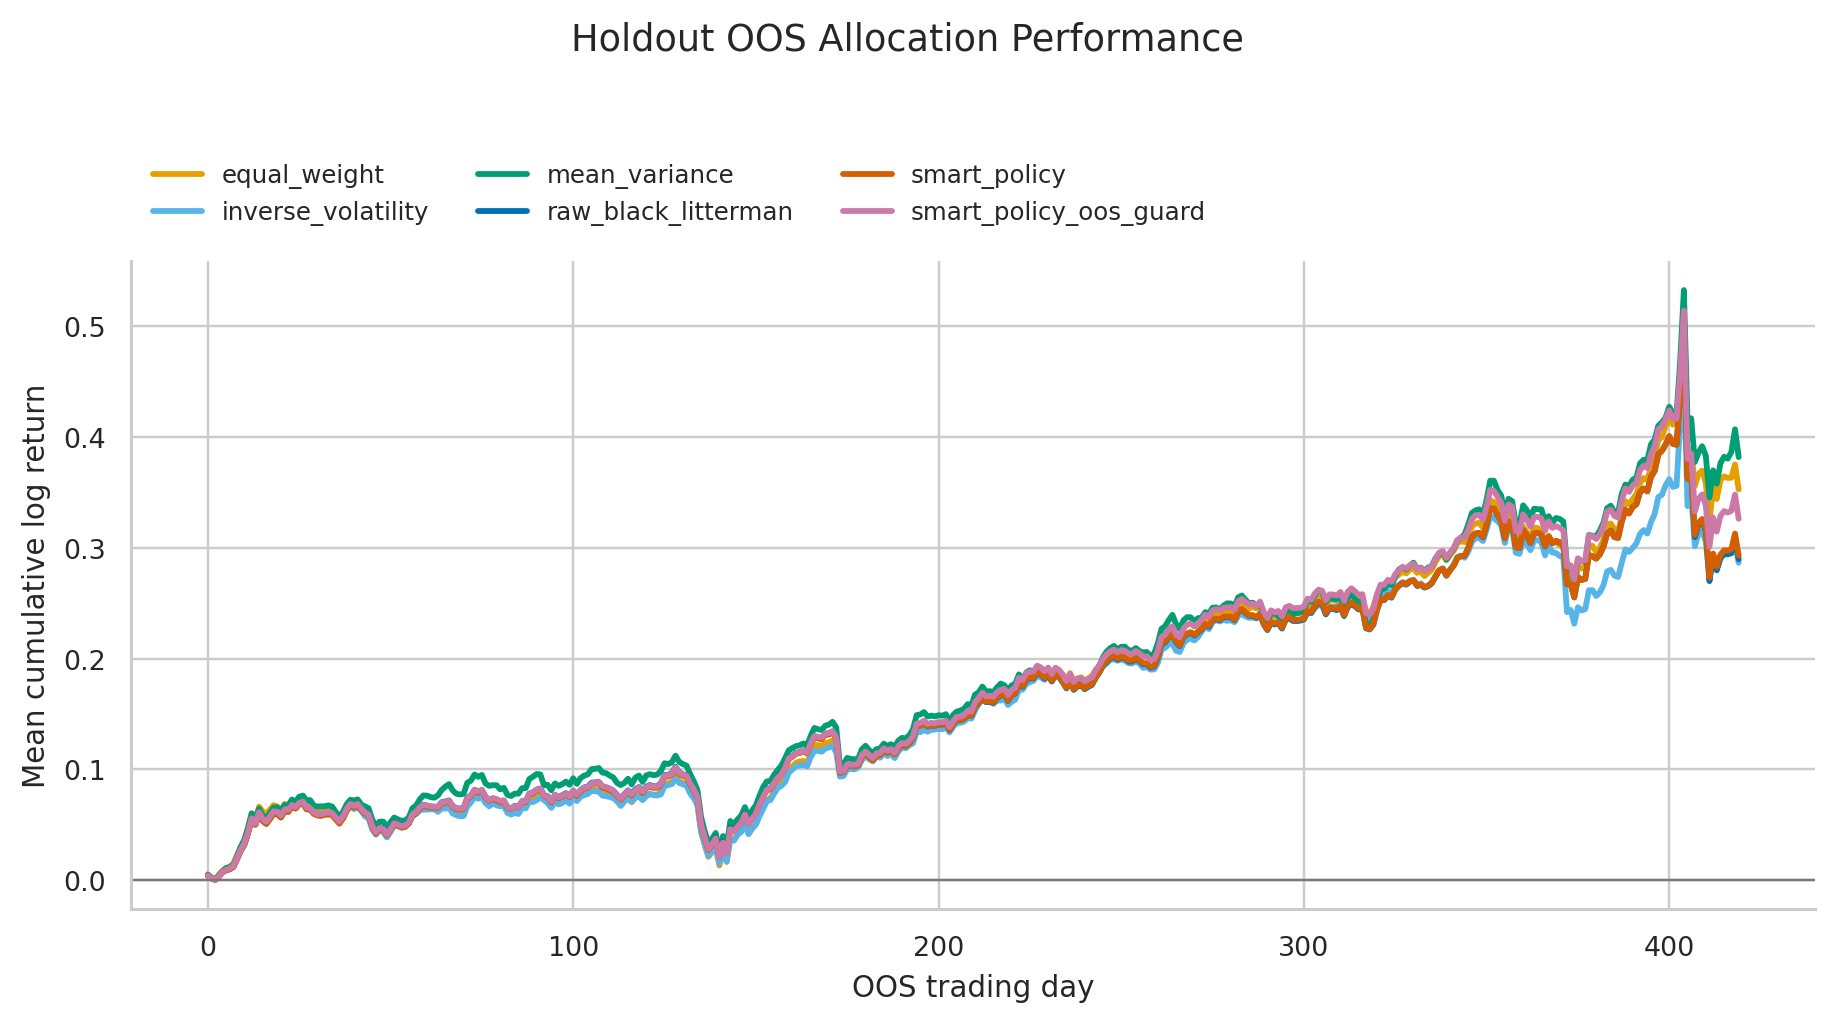
\includegraphics[width=0.88\textwidth]{allocation_oos_curves.png}
  \caption{Mean OOS cumulative log-return curves for allocation strategies across 19 evaluated real-data holdout portfolios, 114 strategy rows, and 42,420 return rows with sandbox disabled. The figure should be read with Table~\ref{tab:allocation} because all strategies have negative mean benchmark excess return.}
  \label{fig:allocation}
\end{figure*}

\subsection{Ablation Study}
Table~\ref{tab:ablation} and Fig.~\ref{fig:ablation} summarize a strategy-level allocation ablation rather than a component-level causal decomposition. Relative to Smart policy with OOS guard, the largest mean positive cumulative-return delta among non-guard strategies came from mean-variance (+0.0135), but its model-score delta remained negative (-0.4579). Smart policy without the OOS guard had mean cumulative-return delta -0.0194 and model-score delta -0.6474. In this run, the guard acts as a stabilizer, though the evidence is not a causal decomposition of every Smart-policy submodule.

\begin{table}[t]
\caption{Allocation Strategy Ablation}
\label{tab:ablation}
\centering
\scriptsize
\begin{tabularx}{\columnwidth}{Y r r r}
\toprule
Ablation & Port. & $\Delta$ cum. ret. & $\Delta$ score \\
\midrule
Equal weight & 19 & -0.0163 & -1.6421 \\
Inverse volatility & 19 & -0.0571 & -0.9737 \\
Mean-variance & 19 & 0.0135 & -0.4579 \\
Raw Black-Litterman & 19 & -0.0188 & -0.3895 \\
Smart policy & 19 & -0.0194 & -0.6474 \\
Smart policy + OOS guard & 19 & 0.0000 & 0.0000 \\
\bottomrule
\end{tabularx}
\tabnote{Deltas are strategy-level differences relative to Smart policy plus OOS guard on the same allocation run. This is not a component-level causal ablation.}
\end{table}

\begin{figure*}[t]
  \centering
  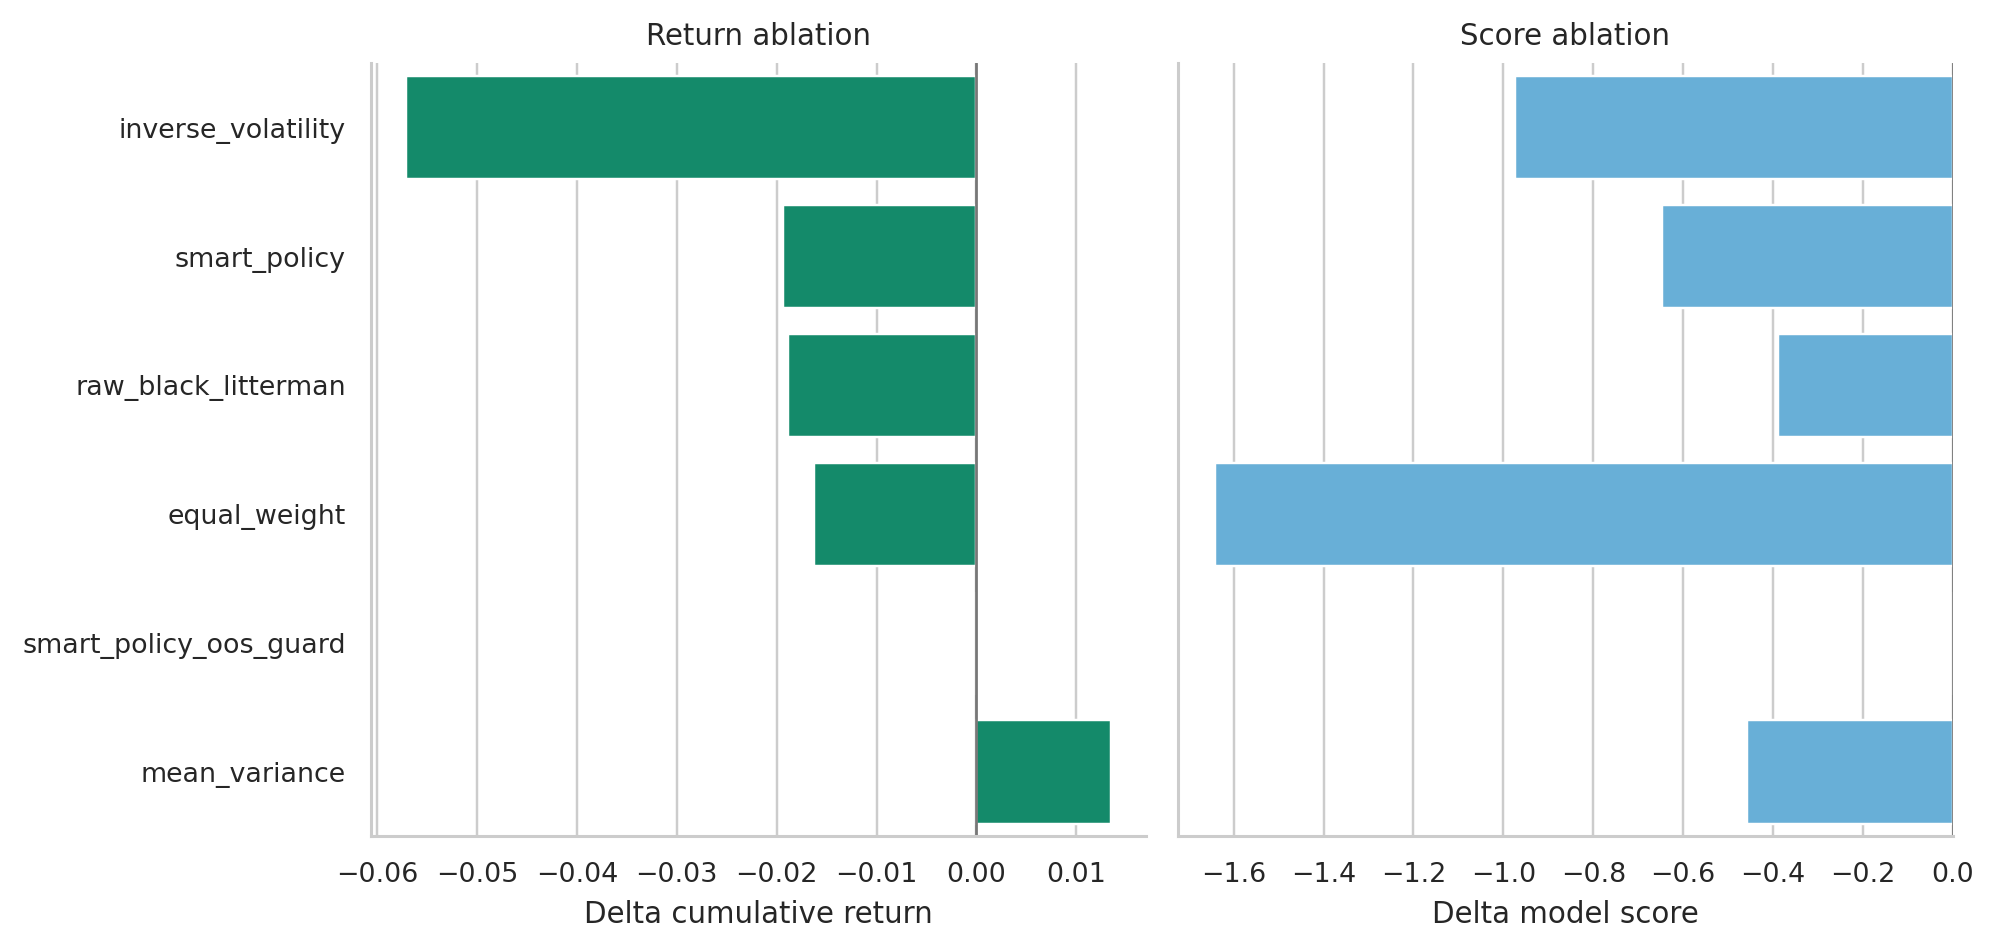
\includegraphics[width=0.85\textwidth]{ablation_summary.png}
  \caption{Coarse strategy-level allocation ablation over the same 19 real-data OOS portfolios used in Fig.~\ref{fig:allocation}. Deltas are relative to Smart policy with OOS guard where present.}
  \label{fig:ablation}
\end{figure*}

\subsection{Statistical Uncertainty}
Table~\ref{tab:uncertainty} adds percentile bootstrap intervals over portfolios, using only saved real-data outputs. For the frozen crisis-warning layer, H1 ROC-AUC was 0.6325 with a cross-portfolio interval of 0.6093 to 0.6533, while H5 ROC-AUC was 0.6325 with an interval of 0.6099 to 0.6511. PR-AUC intervals were narrower in absolute scale but remain modest: 0.0928 to 0.1130 for H1 and 0.0826 to 0.0989 for H5. Allocation intervals are wider because only 19 portfolios are available. Smart policy with OOS guard had mean Sharpe 1.1914 with interval 0.7229 to 1.7184, and mean benchmark excess return -0.1363 with interval -0.2844 to -0.0191. These intervals support the paper's framing as applied evidence for an auditable workflow rather than a claim of universal predictive or allocation strength.

\begin{table*}[t]
\caption{Cross-Portfolio Uncertainty Summary}
\label{tab:uncertainty}
\centering
\scriptsize
\begin{tabularx}{\textwidth}{l Y Y r r r r}
\toprule
Task & Group & Metric & Point & 2.5\% & 97.5\% & Units \\
\midrule
Allocation & Equal weight & Benchmark excess & -0.1526 & -0.2607 & -0.0290 & 19 \\
Allocation & Equal weight & Model score & 58.2789 & 53.7918 & 62.6905 & 19 \\
Allocation & Equal weight & Sharpe & 1.1203 & 0.6804 & 1.7249 & 19 \\
Allocation & Inverse volatility & Benchmark excess & -0.1934 & -0.3236 & -0.0675 & 19 \\
Allocation & Inverse volatility & Model score & 58.9474 & 52.8846 & 63.8063 & 19 \\
Allocation & Inverse volatility & Sharpe & 1.1255 & 0.6678 & 1.6284 & 19 \\
Allocation & Mean-variance & Benchmark excess & -0.1228 & -0.2650 & 0.0222 & 19 \\
Allocation & Mean-variance & Model score & 59.4632 & 53.7747 & 64.5650 & 19 \\
Allocation & Mean-variance & Sharpe & 1.1799 & 0.7092 & 1.7992 & 19 \\
Allocation & Raw Black-Litterman & Benchmark excess & -0.1551 & -0.2926 & -0.0299 & 19 \\
Allocation & Raw Black-Litterman & Model score & 59.5316 & 54.5228 & 64.2830 & 19 \\
Allocation & Raw Black-Litterman & Sharpe & 1.1581 & 0.7008 & 1.7749 & 19 \\
Allocation & Smart policy & Benchmark excess & -0.1557 & -0.2897 & -0.0232 & 19 \\
Allocation & Smart policy & Model score & 59.2737 & 54.2629 & 64.1968 & 19 \\
Allocation & Smart policy & Sharpe & 1.1531 & 0.7033 & 1.8442 & 19 \\
Allocation & Smart policy + OOS guard & Benchmark excess & -0.1363 & -0.2844 & -0.0191 & 19 \\
Allocation & Smart policy + OOS guard & Model score & 59.9211 & 55.2555 & 65.1578 & 19 \\
Allocation & Smart policy + OOS guard & Sharpe & 1.1914 & 0.7229 & 1.7184 & 19 \\
Crisis & H1 & Brier score & 0.0498 & 0.0482 & 0.0514 & 19 \\
Crisis & H1 & Log-loss & 0.2047 & 0.1996 & 0.2095 & 19 \\
Crisis & H1 & PR-AUC & 0.1020 & 0.0928 & 0.1130 & 19 \\
Crisis & H1 & ROC-AUC & 0.6325 & 0.6093 & 0.6533 & 19 \\
Crisis & H1 & Top-decile lift & 2.2988 & 2.0902 & 2.5203 & 19 \\
Crisis & H5 & Brier score & 0.0527 & 0.0509 & 0.0545 & 19 \\
Crisis & H5 & Log-loss & 0.2181 & 0.2087 & 0.2283 & 19 \\
Crisis & H5 & PR-AUC & 0.0904 & 0.0826 & 0.0989 & 19 \\
Crisis & H5 & ROC-AUC & 0.6325 & 0.6099 & 0.6511 & 19 \\
Crisis & H5 & Top-decile lift & 1.9013 & 1.8472 & 2.3705 & 19 \\
\bottomrule
\end{tabularx}
\tabnote{Intervals are 2.5th to 97.5th percentile cross-portfolio bootstrap intervals over saved real-data outputs. Crisis rows resample portfolios within each horizon without retraining frozen artifacts. Allocation rows resample portfolio-level OOS metric rows within each strategy.}
\end{table*}

\subsection{Paired Delta Checks}
The generated paired-delta summary further separates evidence that survives same-portfolio comparison from evidence that is only directional. The crisis-warning deltas show a sharp tradeoff between calibration and ranking: calibrated XGBoost has favorable paired Brier and log-loss deltas against raw XGBoost, but raw scores retain higher PR-AUC at both horizons while ROC-AUC deltas are only directional in this refreshed run. For allocation, Smart policy with OOS guard has favorable paired deltas against unguarded Smart policy for Sharpe, model score, benchmark excess return, and turnover, but its edge against mean-variance is not stable for benchmark excess return or Sharpe.

\begin{table*}[t]
\caption{Selected Paired Delta Checks}
\label{tab:paired-delta}
\centering
\scriptsize
\begin{tabularx}{\textwidth}{l Y Y r r r Y}
\toprule
Family & Reference vs. comparator & Metric & $\Delta$ & 2.5\% & 97.5\% & Reading \\
\midrule
Crisis H1 & Calibrated XGBoost vs. raw XGBoost & PR-AUC & -0.0087 & -0.0159 & -0.0053 & Raw PR ranking is higher. \\
Crisis H1 & Calibrated XGBoost vs. raw XGBoost & Brier score & 0.1580 & 0.1503 & 0.1669 & Calibration improves probability loss. \\
Crisis H5 & Calibrated XGBoost vs. raw XGBoost & ROC-AUC & -0.0108 & -0.0250 & 0.0033 & Directional raw ROC edge only. \\
Crisis H5 & Calibrated XGBoost vs. raw XGBoost & Log-loss & 0.4098 & 0.3876 & 0.4302 & Calibration improves probability loss. \\
Allocation & Guarded Smart vs. Smart & Sharpe & 0.0383 & 0.0176 & 0.0622 & Favorable in paired portfolios. \\
Allocation & Guarded Smart vs. Smart & Benchmark excess & 0.0194 & 0.0076 & 0.0360 & Less negative, not positive in level. \\
Allocation & Guarded Smart vs. Smart & Turnover & 1.2929 & 1.0223 & 1.5471 & Guard reduces turnover. \\
Allocation & Guarded Smart vs. mean-variance & Benchmark excess & -0.0135 & -0.0585 & 0.0289 & No stable paired edge. \\
Allocation & Guarded Smart vs. mean-variance & Turnover & 2.1059 & 1.6616 & 2.5283 & Guard reduces turnover. \\
Allocation & Guarded Smart vs. equal weight & Turnover & -0.3701 & -0.4655 & -0.2835 & Equal weight remains mechanically lower turnover. \\
\bottomrule
\end{tabularx}
\tabnote{Paired deltas use saved outputs joined by portfolio and bootstrap resampled with 500 draws. Positive deltas are oriented so that positive means the reference is better; for Brier score, log-loss, and turnover, the script computes comparator minus reference. Intervals crossing zero are treated as suggestive only.}
\end{table*}

\section{Discussion}
\label{sec:discussion}

\subsection{What the Framework Demonstrates}
The experiments show a narrow but useful point: a multi-market financial ML workflow can be organized around frozen artifacts, hash verification, schema audit, provenance logs, explainable warning drivers, threshold-sensitivity diagnostics, and leakage-guarded allocation evaluation. The result is a reviewable model-risk workflow, not a claim that the chosen XGBoost artifacts or allocation policies are uniquely strong. Modest predictive signals can still be operationally useful when they are presented as ranking surveillance with calibration diagnostics, threshold limitations, and data availability constraints.

\subsection{What It Does Not Demonstrate}
The paper does not demonstrate a consistently dominant tail-risk predictor or establish alpha generation. The main holdout is not a strict zero-security-overlap transfer test, because several holdout portfolios share some constituents with training-domain portfolios. Nor does the allocation study prove that Smart policy is always better than simpler rules; in this run, benchmark excess return is negative for all evaluated strategies.

\subsection{Limitations and Boundary Conditions}
Both frozen crisis-warning artifacts carry \path{degraded_validation} status. This status is not a cosmetic caveat: it means the artifacts should be treated as weak frozen systems used to test auditability and downstream controls, not as deployable warning engines.

The default 0.60 warning threshold has extremely weak recall in the real-data holdout. It flags only 11 rows globally and no H5 rows, so it should not be deployed as a recall-sensitive crisis trigger without recalibration, threshold tuning, and cost-sensitive evaluation. The more defensible interpretation is ranking surveillance, where top-score portfolios form a review queue rather than an automated alarm.

The main holdout is portfolio-level external validation, not a fully zero-security-overlap transfer test. Several holdout portfolios share some individual constituents with the training-domain portfolios. The appendix transfer check is the only zero-security-overlap evidence. Baseline comparison, allocation OOS, and allocation ablation were not run for this panel; therefore, the zero-security-overlap evidence is limited to crisis-warning transfer behavior.

The real-data evidence remains exposed to provider and data drift. Provider availability, symbol mapping, corporate actions, late corrections, trading-calendar handling, and regional market microstructure can change over time. The audit contract can also fail through artifact dependency mismatch, including missing artifact files, schema-hash mismatch, package-version changes, XGBoost native-contribution behavior, or provider API changes.

The explanation layer uses SHAP-style/native XGBoost contribution values. These contributions explain model output for audited rows, but they are not causal estimates of market mechanisms or stress-test variables. The allocation layer is a decision-support and model-risk-management tool, not investment advice. Automated allocation can concentrate losses, amplify model errors, and create false confidence if warnings are presented without uncertainty, provenance, and human oversight.

\section{Conclusion}
\label{sec:conclusion}
This paper presented an auditable explainable AI framework for multi-market tail-risk warning and leakage-guarded Bayesian portfolio allocation. Across US, HK, CN, JP, and TW holdout portfolios, frozen XGBoost artifacts produced modest crisis-warning ranking performance, while calibration improved probability quality. Threshold sensitivity showed that the default 0.60 operating point is too conservative for recall, so the warning layer is better read as ranking surveillance. The allocation experiments showed guarded decision discipline, including lower turnover than unguarded Smart policy and raw Black-Litterman, but mean benchmark excess return remained negative. The main contribution is an artifact-backed framework for auditability, reproducibility, leakage control, and honest applied validation, not a claim of predictive dominance.

Future work should expand the holdout pool, add richer macro and cross-asset factors, develop market-specific factor models, introduce online drift monitoring, and strengthen calibration and threshold selection under explicit cost functions.

\appendices
\section{Zero-Security-Overlap Crisis-Warning Details}
\label{app:zero-overlap}
The zero-security-overlap transfer check evaluates only the frozen crisis-warning artifacts. Baseline comparison, allocation OOS, and allocation ablation were not run for this panel; therefore, the zero-security-overlap evidence is limited to crisis-warning transfer behavior. The transfer check produced 36,114 prediction rows with sandbox disabled and zero skipped crisis-warning rows. Table~\ref{tab:zero-crisis} reports the market-level metrics.

\begin{table*}[t]
\caption{Zero-Security-Overlap Crisis-Warning Metrics}
\label{tab:zero-crisis}
\centering
\scriptsize
\begin{tabularx}{\textwidth}{c c r r r r r r r}
\toprule
H & Market & Rows & Pos. & ROC & PR & Brier & Recall@0.60 & Top-decile lift \\
\midrule
1 & CN & 3,926 & 184 & 0.5699 & 0.0600 & 0.0446 & 0.0000 & 1.6288 \\
1 & HK & 3,990 & 202 & 0.6236 & 0.0954 & 0.0471 & 0.0000 & 2.1287 \\
1 & JP & 3,935 & 209 & 0.6465 & 0.1096 & 0.0493 & 0.0000 & 2.7716 \\
1 & TW & 2,162 & 129 & 0.6236 & 0.0952 & 0.0558 & 0.0000 & 2.0081 \\
1 & US & 4,084 & 210 & 0.6731 & 0.1325 & 0.0470 & 0.0190 & 2.6152 \\
5 & CN & 3,910 & 196 & 0.5699 & 0.0670 & 0.0475 & 0.0000 & 1.8878 \\
5 & HK & 3,974 & 231 & 0.5910 & 0.1032 & 0.0536 & 0.0000 & 2.0748 \\
5 & JP & 3,919 & 240 & 0.6334 & 0.1012 & 0.0566 & 0.0000 & 2.2494 \\
5 & TW & 2,146 & 138 & 0.6182 & 0.0873 & 0.0601 & 0.0000 & 1.5912 \\
5 & US & 4,068 & 228 & 0.6527 & 0.1011 & 0.0521 & 0.0000 & 2.1919 \\
\bottomrule
\end{tabularx}
\tabnote{Metrics use 36,114 real-data zero-security-overlap holdout predictions with sandbox disabled across 1D and 5D horizons. No crisis-warning rows were skipped.}
\end{table*}

\clearpage

\raggedbottom

\section*{Data and Code Availability}
The reproducibility package contains the source code, experiment scripts and configs, frozen H1/H5 crisis-warning artifacts, generated result CSV/JSON files, paper tables, figures, the SHA-256 result manifest, and the reproducibility README. The public paper artifact repository is available at \url{https://github.com/Elvin-Chow/DeepFirm-Quant_Paper-Artifact-Repository}. The submitted artifact version is identified by release tag \texttt{v0.1-submission}. An archival DOI will be provided through a release archive when available. Real-market data were accessed through live providers such as Yahoo Finance and AKShare and are documented through generated outputs, provenance fields, and skip logs rather than redistributed as a raw vendor dataset. Paper metrics use sandbox data disabled; provider failures are reported in the data availability log instead of being filled with synthetic data.

\section*{Funding}
This research received no external funding and was self-funded by the author.

\section*{Conflicts of Interest}
The author declares no conflicts of interest.

\section*{AI-Use Disclosure}
The author used OpenAI Codex to assist with manuscript drafting and editing, code review, and efficient experiment execution and verification. The author reviewed, revised, and approved the final manuscript text, code changes, analyses, and reported results.

\clearpage

\bibliographystyle{IEEEtran}
\bibliography{../references}

\begin{IEEEbiographynophoto}{Hongyi Zhou}
Hongyi Zhou is an undergraduate student in Information Systems and Web Technologies at the School of Professional Education and Executive Development, The Hong Kong Polytechnic University, Hong Kong. His interests include financial research, software implementation, frontend design, and photography.
\end{IEEEbiographynophoto}

\EOD
\end{document}
